\documentclass{standalone}

\usepackage{tikz}
\usepackage{amsmath, amssymb,stackrel}

%% Public TikZ libraries
\usetikzlibrary{arrows}
\usetikzlibrary{calc}
\usetikzlibrary{circuits.logic.US}
\usetikzlibrary{positioning}
\usetikzlibrary{shapes}
\usetikzlibrary{decorations.pathreplacing}

\newcommand\aCipher{\textsc{Sparkle}}
\newcommand\aCipherSmall{\textsc{Sparkle256}}
\newcommand\aCipherMedium{\textsc{Sparkle384}}
\newcommand\aCipherLarge{\textsc{Sparkle512}}
\newcommand\aead{\textsc{Schwaemm}}
\newcommand\hash{\textsc{Esch}}
\newcommand\wordSpace{\mathbb{W}}
\newcommand\branchSpace{\mathbb{B}}
\newcommand\branches{n_b}
\newcommand\halfbranches{h_b}
\newcommand\steps{n_s}
\newcommand\roundsPerStep{r_{s}}
\newcommand\arxbox{A}
\newcommand\difflayer{\mathcal{L}}
\newcommand\linFeist[1]{\mathcal{M}_{ #1 }}
\newcommand\boundProbaPartial[1]{\mathsf{P}_{\mathsf{vanish}}(#1)}
\newcommand\constIterator{\rho}
\newcommand\arxround{\mathcal{R}}

%% Custom TikZ addons
	
%% Document

\begin{document}


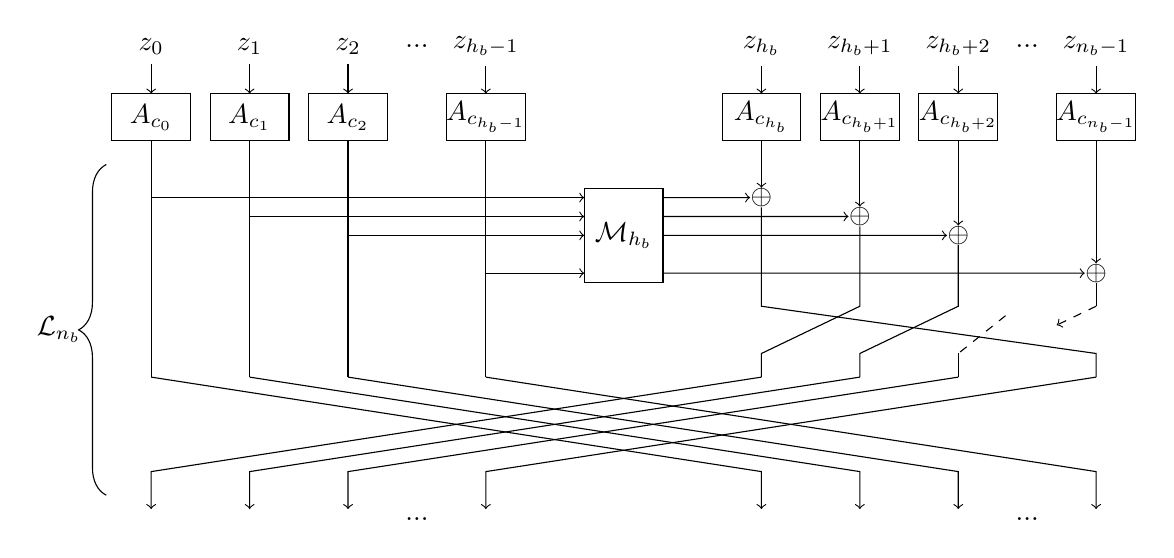
\begin{tikzpicture}[xscale=0.5, yscale=0.6]
    %% input
    \draw (-12.0, +5.0) node(x0){$z_0$} ;
    \draw (-9.5, +5.0) node(x1){$z_1$} ;
    \draw (-7.0, +5.0) node(x2){$z_2$} ;
    \draw (-5.25, +5.0) node{...} ;
    \draw (-3.5, +5.0) node(xB){$z_{\halfbranches-1}$} ;
    \draw (+3.5, +5.0) node(y0){$z_{\halfbranches}$} ;
    \draw (+6.0, +5.0) node(y1){$z_{\halfbranches+1}$} ;
    \draw (+8.5, +5.0) node(y2){$z_{\halfbranches+2}$} ;
    \draw (+10.25, +5.0) node{...} ;
    \draw (+12.0, +5.0) node(yB){$z_{\branches-1}$} ;
    \draw [->] (x0) -- (-12.0, 4) ;
    \draw [->] (x1) -- (-9.5, 4) ;
    \draw [->] (x2) -- (-7.0, 4) ;
    \draw [->] (xB) -- (-3.5, 4) ;
    \draw [->] (y0) -- (+3.5, 4) ;
    \draw [->] (y1) -- (+6.0, 4) ;
    \draw [->] (y2) -- (+8.5, 4) ;
    \draw [->] (yB) -- (+12.0, 4) ;
    %% ARXboxes
    \draw (-13.0, 3) rectangle (-11.0, 4) node[pos=0.5]{$\arxbox_{c_0}$} ;
    \draw (-10.5, 3) rectangle (-8.5, 4) node[pos=0.5]{$\arxbox_{c_1}$} ;
    \draw (-8.0, 3) rectangle (-6.0, 4) node[pos=0.5]{$\arxbox_{c_2}$} ;
    \draw (-4.5, 3) rectangle (-2.5, 4) node[pos=0.5]{$\arxbox_{c_{\halfbranches-1}}$} ;
    \draw (+2.5, 3) rectangle (+4.5, 4) node[pos=0.5]{$\arxbox_{c_{\halfbranches}}$} ;
    \draw (+5.0, 3) rectangle (+7.0, 4) node[pos=0.5]{$\arxbox_{c_{\halfbranches+1}}$} ;
    \draw (+7.5, 3) rectangle (+9.5, 4) node[pos=0.5]{$\arxbox_{c_{\halfbranches+2}}$} ;
    \draw (+11.0, 3) rectangle (+13.0, 4) node[pos=0.5]{$\arxbox_{c_{\branches-1}}$} ;
    %% Feistel function
    \draw (-1, 0) rectangle (1, 2) node[pos=0.5]{$\linFeist{\halfbranches}$} ;
    \draw (+3.5, 1.8) node[inner sep=0](xor0){$\oplus$} ;
    \draw (+6.0, 1.4) node[inner sep=0](xor1){$\oplus$} ;
    \draw (+8.5, 1.0) node[inner sep=0](xor2){$\oplus$} ;
    \draw (+12.0, 0.2) node[inner sep=0](xorB){$\oplus$} ;
    %% -- arrows from the Feistel function
    \draw[->] (1, 1.8) -- (xor0) ;
    \draw[->] (1, 1.4) -- (xor1) ;
    \draw[->] (1, 1.0) -- (xor2) ;
    \draw[->] (1, 0.2) -- (xorB) ;
    %% -- arrows to the Feistel function
    \draw[->] (-12.0, 1.8) -- (-1, 1.8);
    \draw[->] (-9.5, 1.4) -- (-1, 1.4);
    \draw[->] (-7.0, 1.0) -- (-1, 1.0);
    \draw[->] (-3.5, 0.2) -- (-1, 0.2);
    %% -- arrows down from the ARXboxes
    %% -- -- left
    \draw (-12.0, 3) -- (-12.0, -2);
    \draw (-9.5, 3) -- (-9.5, -2);
    \draw (-7.0, 3) -- (-7.0, -2);
    \draw (-3.5, 3) -- (-3.5, -2);
    %% -- -- right
    \draw[->] (3.5, 3) -- (xor0);
    \draw[->] (6, 3) -- (xor1);
    \draw[->] (8.5, 3) -- (xor2); 
    \draw[->] (12.0, 3) -- (xorB);
    \draw (xor0) -- (3.5, -0.5) -- (12.0, -1.5) -- (12.0, -2) ;
    \draw (xor1) -- (6, -0.5) -- (3.5, -1.5) -- (3.5, -2) ;
    \draw (xor2) -- (8.5, -0.5) -- (6, -1.5) -- (6, -2) ;
    \draw (xorB) -- (12, -0.5) ;
    \draw[style=dashed,->] (12, -0.5) -- (11.0, -0.9) ;
    \draw[style=dashed] (9.7, -0.7) -- (8.5, -1.5) ;
    \draw (8.5, -1.5) -- (8.5, -2) ;
    %% Final swap
    %% -- outputs
    \draw (-12.0, -5.0) node(x0end){} ;
    \draw (-9.5, -5.0) node(x1end){} ;
    \draw (-7.0, -5.0) node(x2end){} ;
    \draw (-5.25, -5.0) node{...} ;
    \draw (-3.5, -5.0) node(xBend){} ;
    \draw (+3.5, -5.0) node(y0end){} ;
    \draw (+6.0, -5.0) node(y1end){} ;
    \draw (+8.5, -5.0) node(y2end){} ;
    \draw (+10.25, -5.0) node{...} ;
    \draw (+12.0, -5.0) node(yBend){} ;   
    %% -- left to right
    \draw[->] (-12.0, -2) -- (+3.5, -4) -- (y0end);
    \draw[->] (-9.5, -2) -- (+6.0, -4) -- (y1end);
    \draw[->] (-7.0, -2) -- (+8.5, -4) -- (y2end);
    \draw[->] (-3.5, -2) -- (+12.0, -4) -- (yBend);
    %% -- right to left
    \draw[->] (+3.5, -2) -- (-12.0, -4) -- (x0end);
    \draw[->] (+6.0, -2) -- (-9.5, -4) -- (x1end);
    \draw[->] (+8.5, -2) -- (-7.0, -4) -- (x2end);
    \draw[->] (+12.0, -2) -- (-3.5, -4) -- (xBend);
    %% Explanations
    \draw [decorate,decoration={brace,amplitude=10pt},xshift=-4pt,yshift=0pt] (-13,-4.5) -- (-13,2.5) node [black,midway,xshift=-0.6cm] {$\mathcal{L}_{\branches}$};
\end{tikzpicture}
\end{document}
